\documentclass[xcolor=dvipsnames,t,aspectratio=169]{beamer} %t para ficar alinhado no topo do slide

\usecolortheme{rose}
\usecolortheme{dolphin}
\usetheme{Boadilla}

\input{imports}

\input{settings}

\input{commands}



\titlegraphic{
    
\includegraphics[scale = 0.25]{figures/emap_logo.png}
}

\logo{
\begin{tikzpicture}[overlay,remember picture]
\node[left=1.1cm, below=0.2cm] at (current page.30){
    
\includegraphics[width=0.165\textwidth]{figures/emap_logo.png}};
\end{tikzpicture}
}


\lstset{style=mystyle}

\newcommand{\highlight}[1]{{\color{fgv_light_blue} #1}}

\title{Forecasting Dengue in Brazilian Capital Cities}

\author{
    Ezequiel Braga
}

\date{{\color{fgv_dark_blue} \textbf{School of Applied Mathematics, \\ Getulio Vargas Foundation, \\ Rio de Janeiro - RJ}}}

\begin{document}

\frame[plain]{\titlepage}
\setcounter{framenumber}{0}

\begin{frame}[c]{Introduction}

    \begin{display}[Goal]
        We compare forecasting models for weekly dengue incidence in the 27 Brazilian capital cities.
        \begin{itemize}
            \item Evaluate whether climate covariates improve forecasting performance;
            \item Compare three model families: INLA, AR(p), and SARIMAX;
            \item Select the best model in each capital using mean absolute error (MAE) and weighted interval score (WIS).
        \end{itemize}
    \end{display}

\end{frame}

\begin{frame}[c]{Capital Cities Study}{Data and forecasting design}

    \begin{display}[Set-up]
        The analysis is based on weekly dengue counts and climate covariates for each capital city.
        \begin{itemize}
            \item 27 Brazilian capital cities;
            \item Weekly dengue reported cases as the response;
            \item Climate summaries based on lagged moving averages;
            \item Rolling forecasting windows with horizon of 8 weeks;
            \item Train: 2010-2025; Test: 2025-present;
            \item Model comparison based on out-of-sample MAE and WIS.
        \end{itemize}
    \end{display}

\end{frame}

\begin{frame}[c]{Capital Cities Study}{Candidate models}

    \begin{display}[Model families]
        We compare three classes of models:
        \begin{itemize}
            \item \highlight{INLA models} (`M0--M7`): poisson/negbin temporal random effects with optional climate covariates;
            \item \highlight{AR(p)} (`M8`): autoregressive benchmark model;
            \item \highlight{SARIMAX models} (`M9--M13`): time-series models with exogenous climate regressors.
        \end{itemize}
    \end{display}

\end{frame}

\begin{frame}[c]{Capital Cities Study}{Candidate models}

    \begin{display}[Main covariates]
        The climate information enters through lagged summaries such as:
        \begin{itemize}
            \item temperature averaged over 8 or 12 weeks;
            \item minimum and maximum temperature averaged over 8 or 12 weeks;
            \item average maximum humidity over 12 weeks;
            \item average precipitation over 52 weeks.
        \end{itemize}
    \end{display}

\end{frame}

\begin{frame}[c]{Capital Cities Study}{National summary}

    \begin{table}[H]
        \centering
        \begin{tabular}{lc|c}
            \hline
             & MAE & WIS \\
            \hline
            \highlight{SARIMAX} & 11 (40.8\%) & 16 (59.26\%) \\
            \highlight{INLA} & 10 (37.0\%) & 5 (18.54\%) \\
            \highlight{AR(p)} & 6 (22.2\%) & 6 (22.2\%) \\
            \hline
        \end{tabular}
        \caption{Number of capitals where each model wins based on each metric.}
    \end{table}

\end{frame}

\begin{frame}[c]{Capital Cities Study}{National summary}

    \begin{figure}
        \centering
        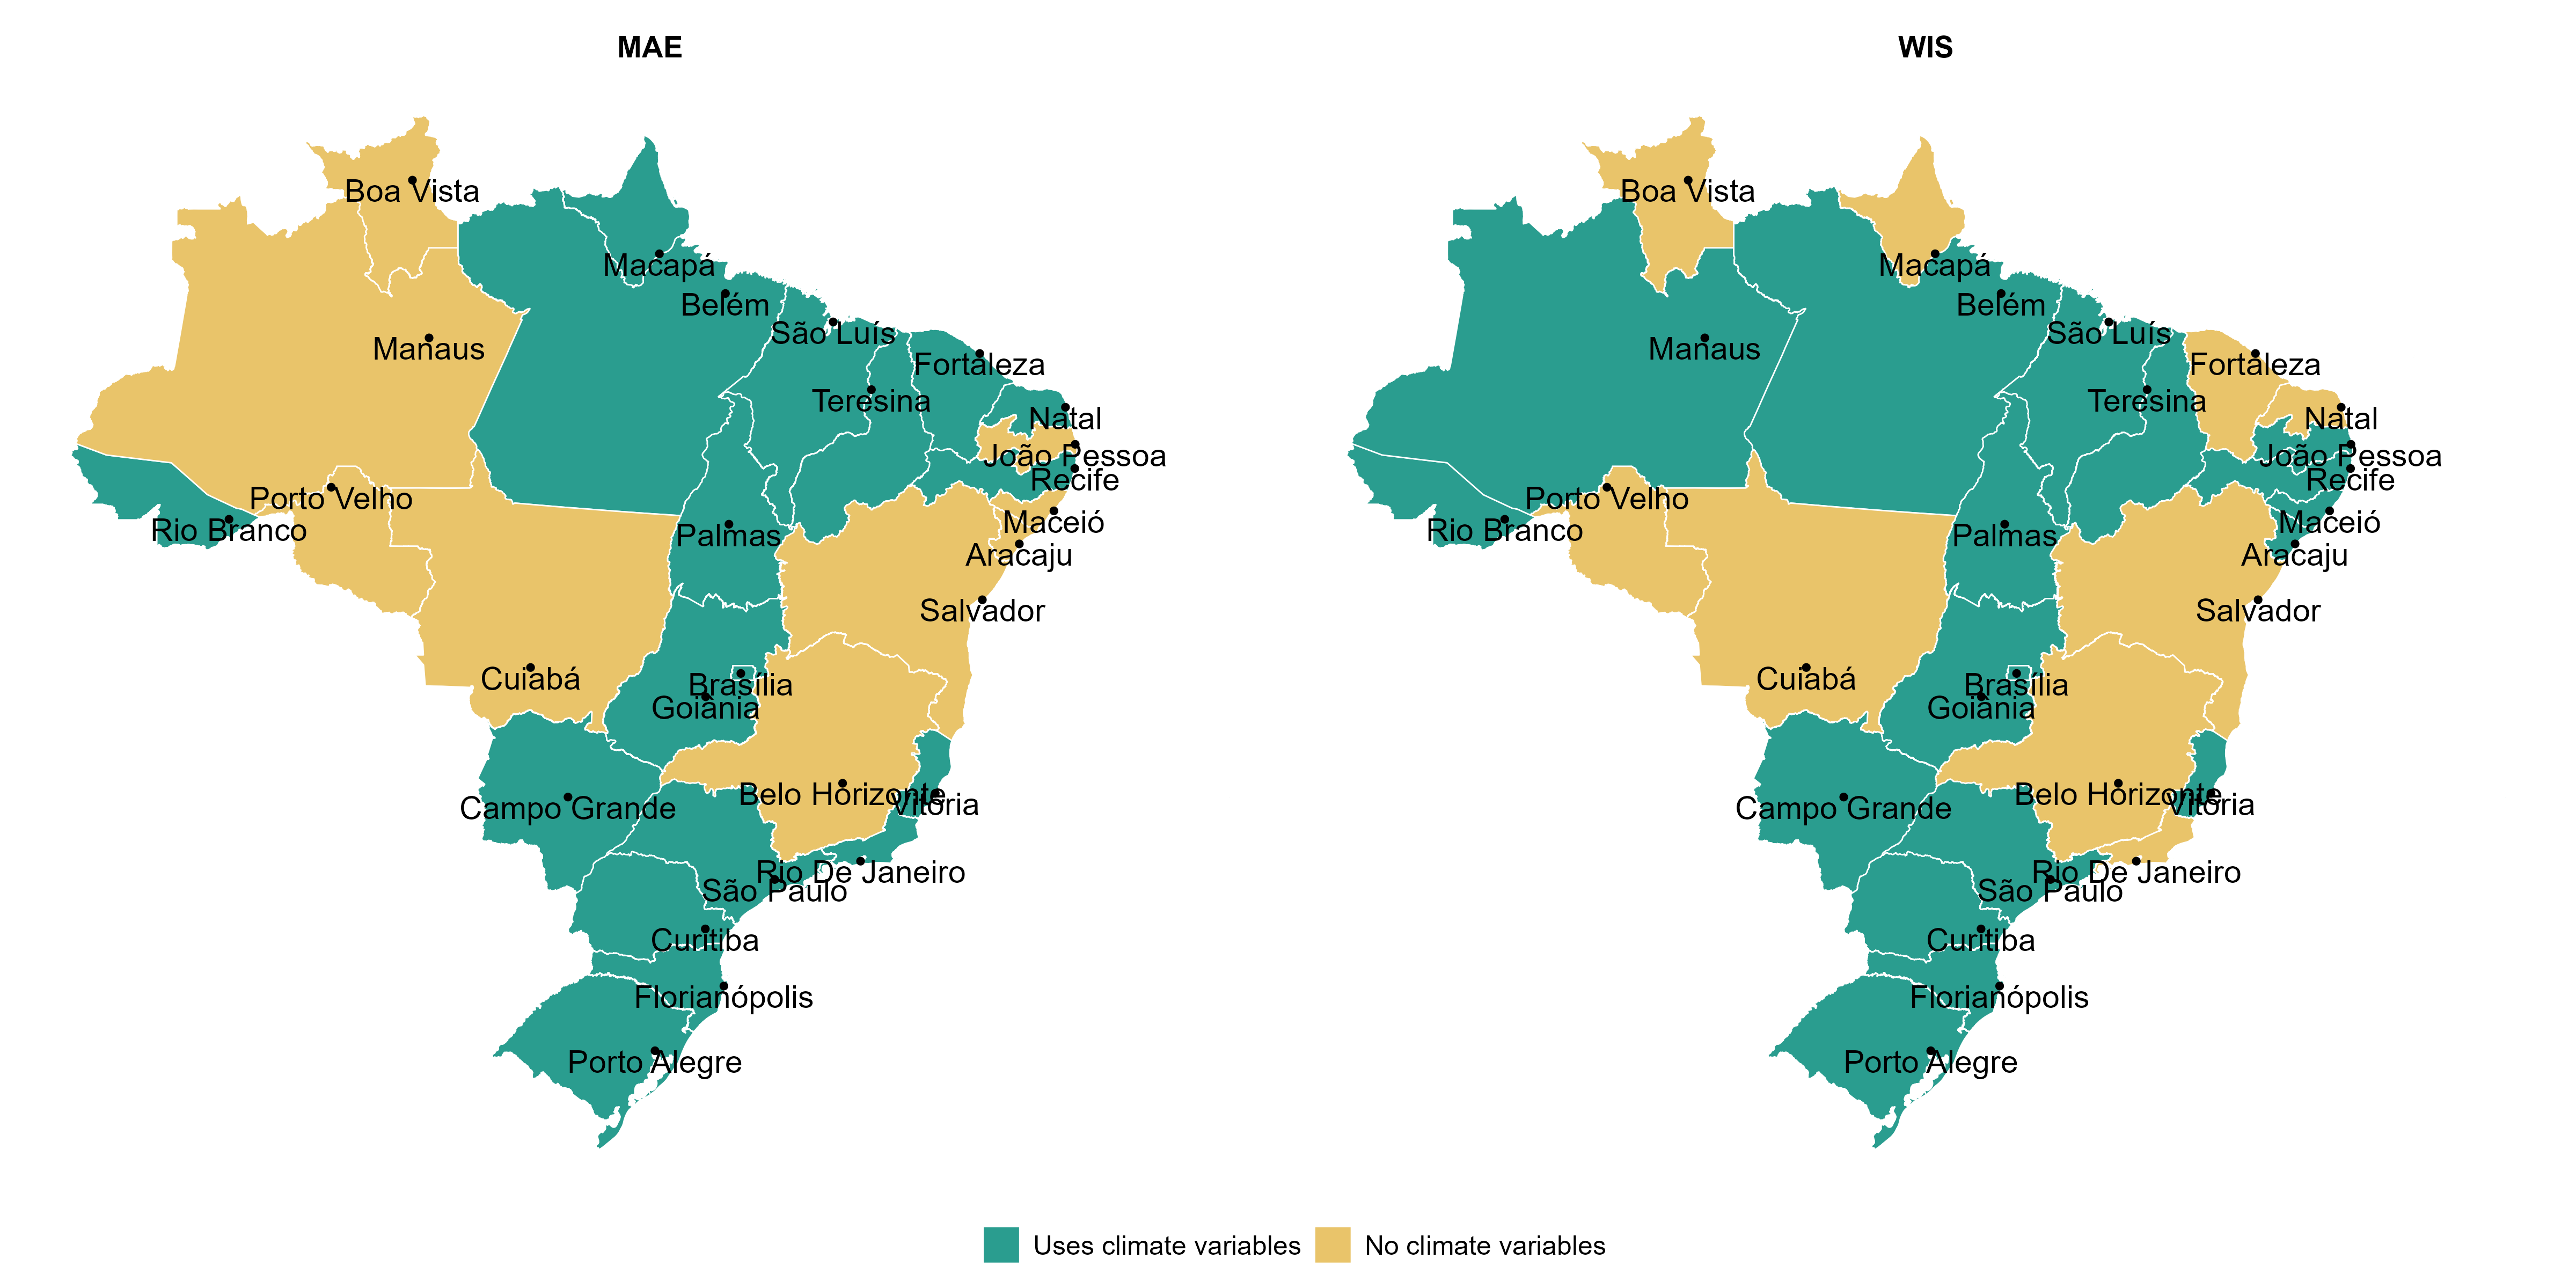
\includegraphics[scale=0.33]{figures/best_model_climate_combined.png}
        \caption{Use of climate variables comparioson based on MAE and WIS.}
        \label{fig:best_model_climate_combined}
    \end{figure}

\end{frame}

\begin{frame}[c]{Capital Cities Study}{National summary}

    \begin{figure}
        \centering
        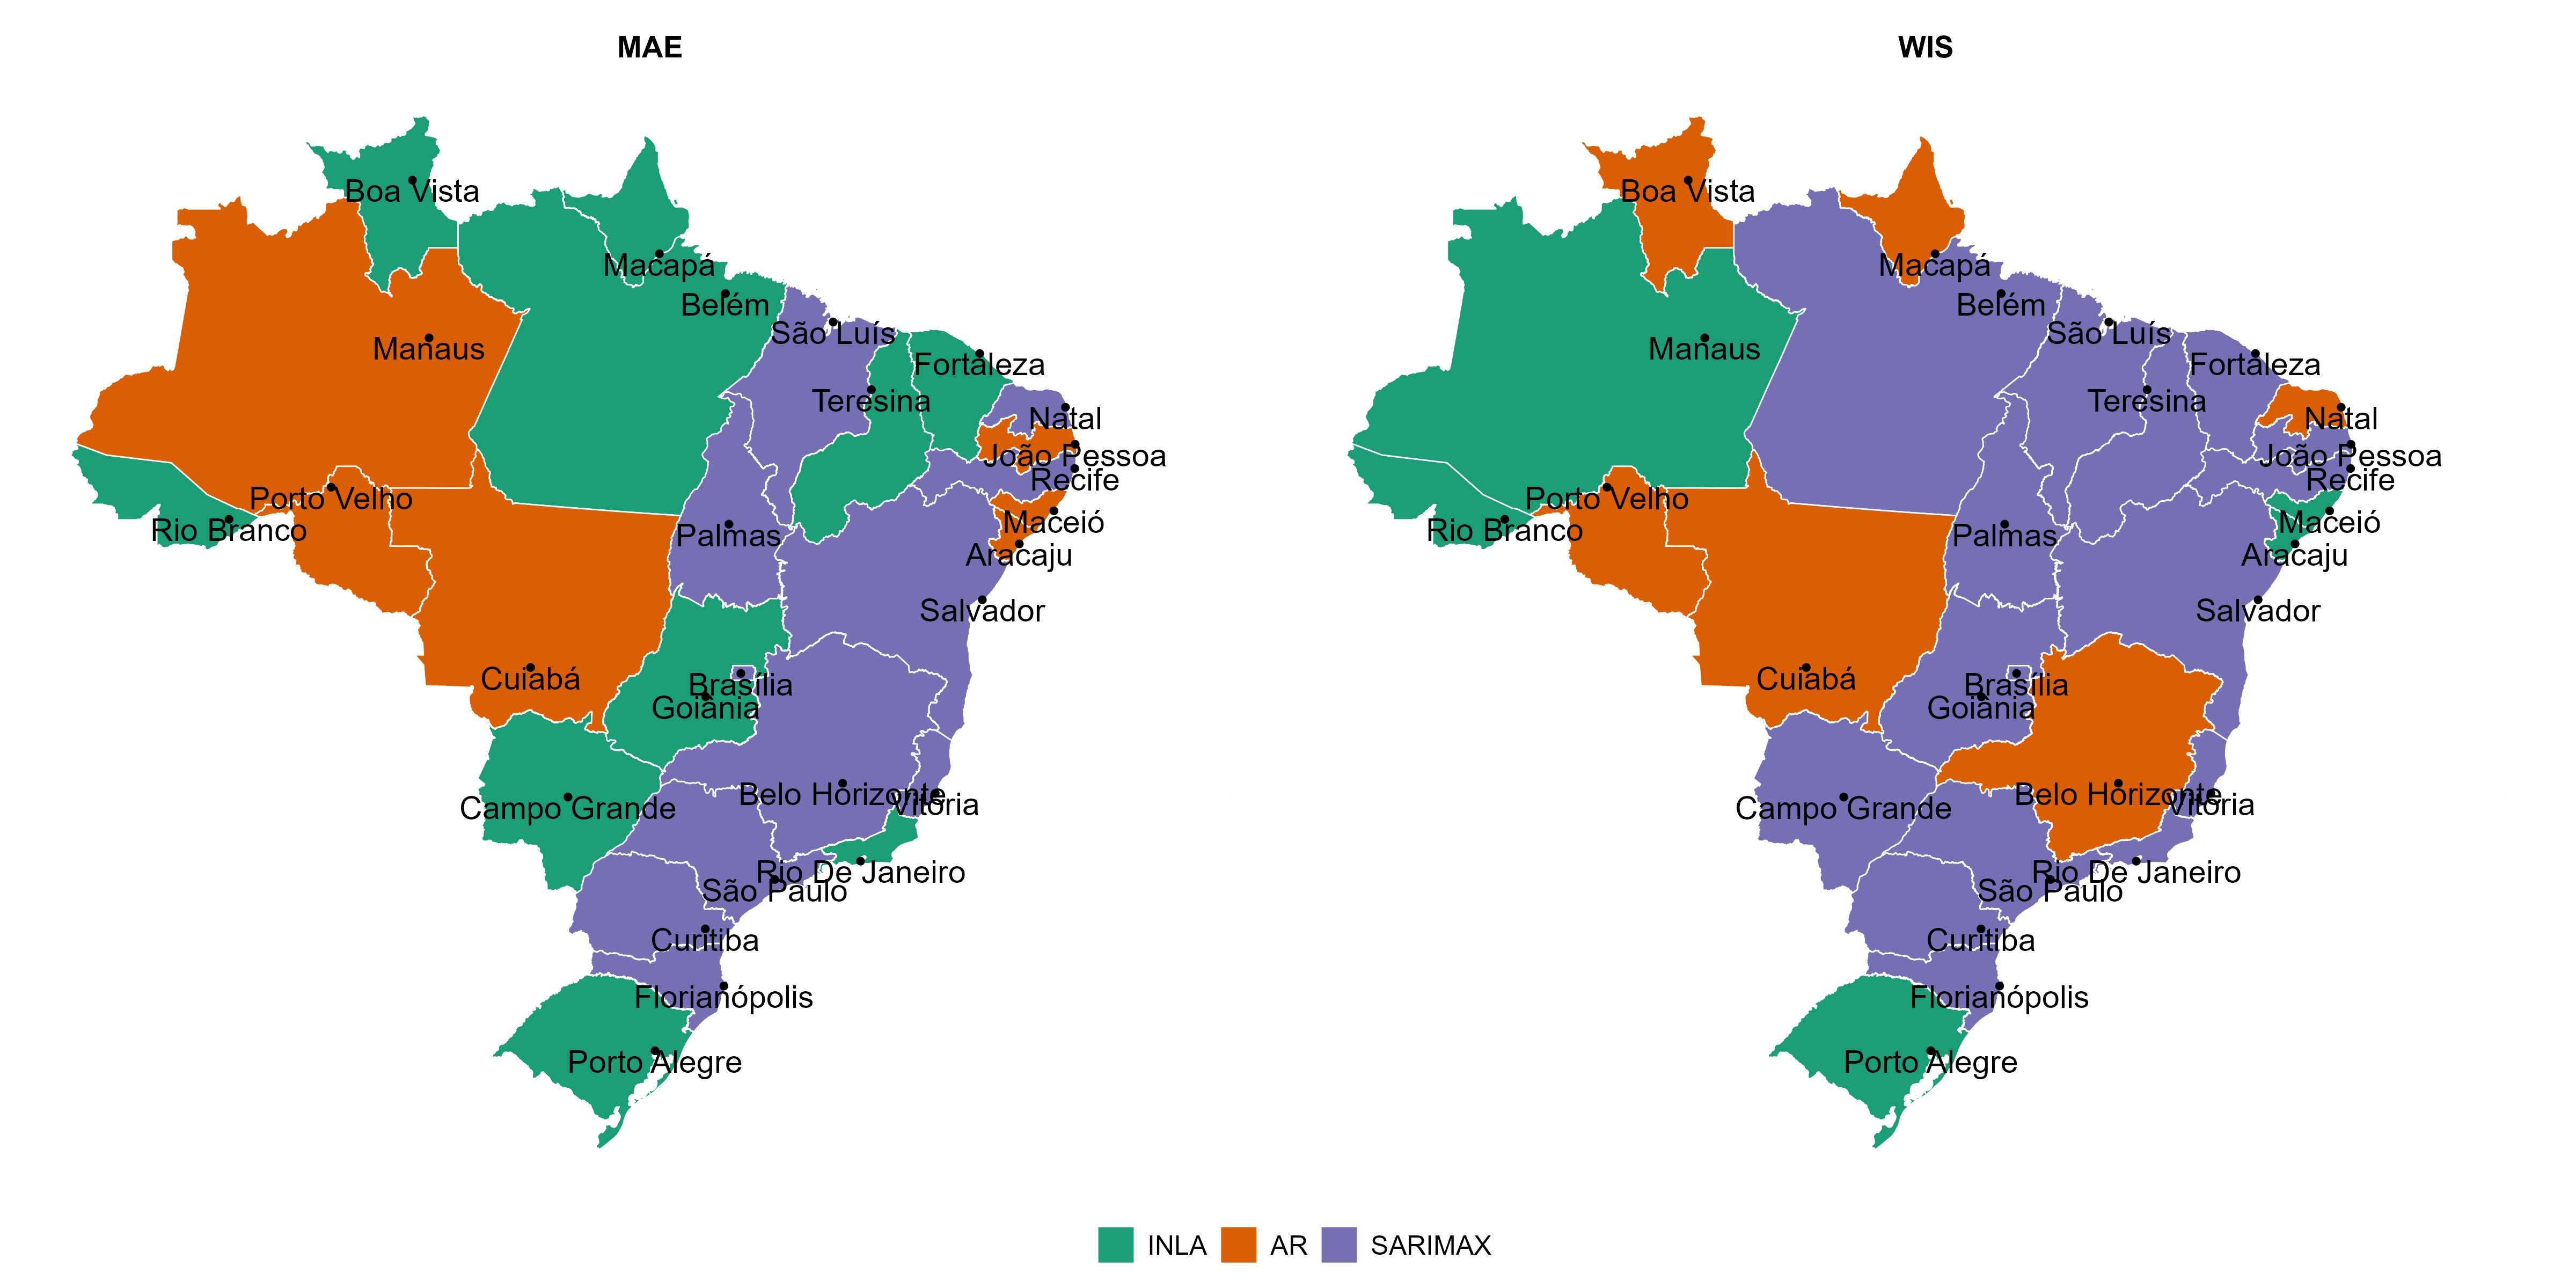
\includegraphics[scale=0.33]{figures/best_model_type_combined.png}
        \caption{Best model type comparison based on MAE and WIS.}
        \label{fig:best_model_type_combined}
    \end{figure}

\end{frame}

\begin{frame}[c]{Capital Cities Study}{Best model by capital}

\scriptsize
\begin{columns}[T]
    \column{0.40\textwidth}
    \begin{display}[SARIMAX winners]
        \begin{table}[H]
            \centering
            \begin{tabular}{l|ll}
                 & MAE & WIS \\
                \hline
                \multirow{3}{*}{M9} 
                 & \highlight{BA} & \highlight{BA} \\
                 & MG & CE \\
                 & & RJ \\
                 \hline
                \multirow{4}{*}{M11} 
                 & \highlight{DF} & \highlight{DF} \\
                 & \highlight{ES} & \highlight{ES} \\
                 & \highlight{PR} & \highlight{PR} \\
                 & & GO \\
                 \hline
                \multirow{5}{*}{M12} 
                 & \highlight{MA} & \highlight{MA} \\
                 & \highlight{PE} & \highlight{PE} \\
                 & RN & PA \\
                 & & PB \\
                 \hline
                 \multirow{5}{*}{M13} 
                 & \highlight{SC} & \highlight{SC} \\
                 & \highlight{TO} & \highlight{TO} \\
                 & \highlight{SP} & \highlight{SP} \\
                 & & MS \\
                 & & PI 
            \end{tabular}
        \end{table}
    \end{display}
    
    \column{0.32\textwidth}
    \begin{display}[INLA winners]
        \begin{table}[H]
            \centering
            \begin{tabular}{l|ll}
                 & MAE & WIS \\
                \hline
                M0 & RR & \\
                \hline
                \multirow{2}{*}{M1} & GO & \\
                 & PA & \\
                 \hline
                \multirow{2}{*}{M3} & CE & AL \\
                 & RJ & \\
                 \hline
                \multirow{2}{*}{M4} & MS & AM \\
                 & PI & \\
                 \hline
                M5 & AP & \\
                \hline
                \multirow{3}{*}{M6} 
                 & \highlight{AC} & \highlight{AC} \\
                 & \highlight{RS} & \highlight{RS} \\
                 & & CE \\
            \end{tabular}
        \end{table}
    \end{display}

    \column{0.28\textwidth}
    \begin{display}[AR winners]
        \begin{table}[H]
            \centering
            \begin{tabular}{l|ll}
                 & MAE & WIS \\
                \hline
                \multirow{6}{*}{M8} 
                 & AL & RR \\
                 & AM & AP \\
                 & \highlight{MT} & \highlight{MT} \\
                 & PB & MG \\
                 & \highlight{RO} & \highlight{RO} \\
                 & SE & RN \\
                 \hline
            \end{tabular}
        \end{table}
    \end{display}
\end{columns}

\end{frame}

% \begin{frame}[c]{Capital Cities Study}{Interpretation of the winners}

%     \begin{display}[What do the results suggest?]
%         The best model varies substantially by capital city.
%         \begin{itemize}
%             \item In several capitals, \highlight{climate-augmented SARIMAX} models give the best forecasts;
%             \item In other capitals, \highlight{INLA} models with structured temporal effects remain competitive;
%             \item In 6 capitals, a simple \highlight{AR(p)} model is the best choice, suggesting that recent dengue history may already capture much of the signal.
%         \end{itemize}
%     \end{display}

% \end{frame}

% \begin{frame}[c]{Capital Cities Study}{Interpretation of the winners}

%     \begin{display}[Climate signal]
%         Among the SARIMAX winners:
%         \begin{itemize}
%             \item precipitation appears in the best model for DF, ES and PR;
%             \item humidity appears in the best model for MA, PE and RN;
%             \item a 12-week temperature average is selected for SC, SP and TO.
%         \end{itemize}
%     \end{display}

% \end{frame}

\begin{frame}[c]{Capital Cities Study}{Forecast accuracy highlights}

    \begin{figure}
        \centering
        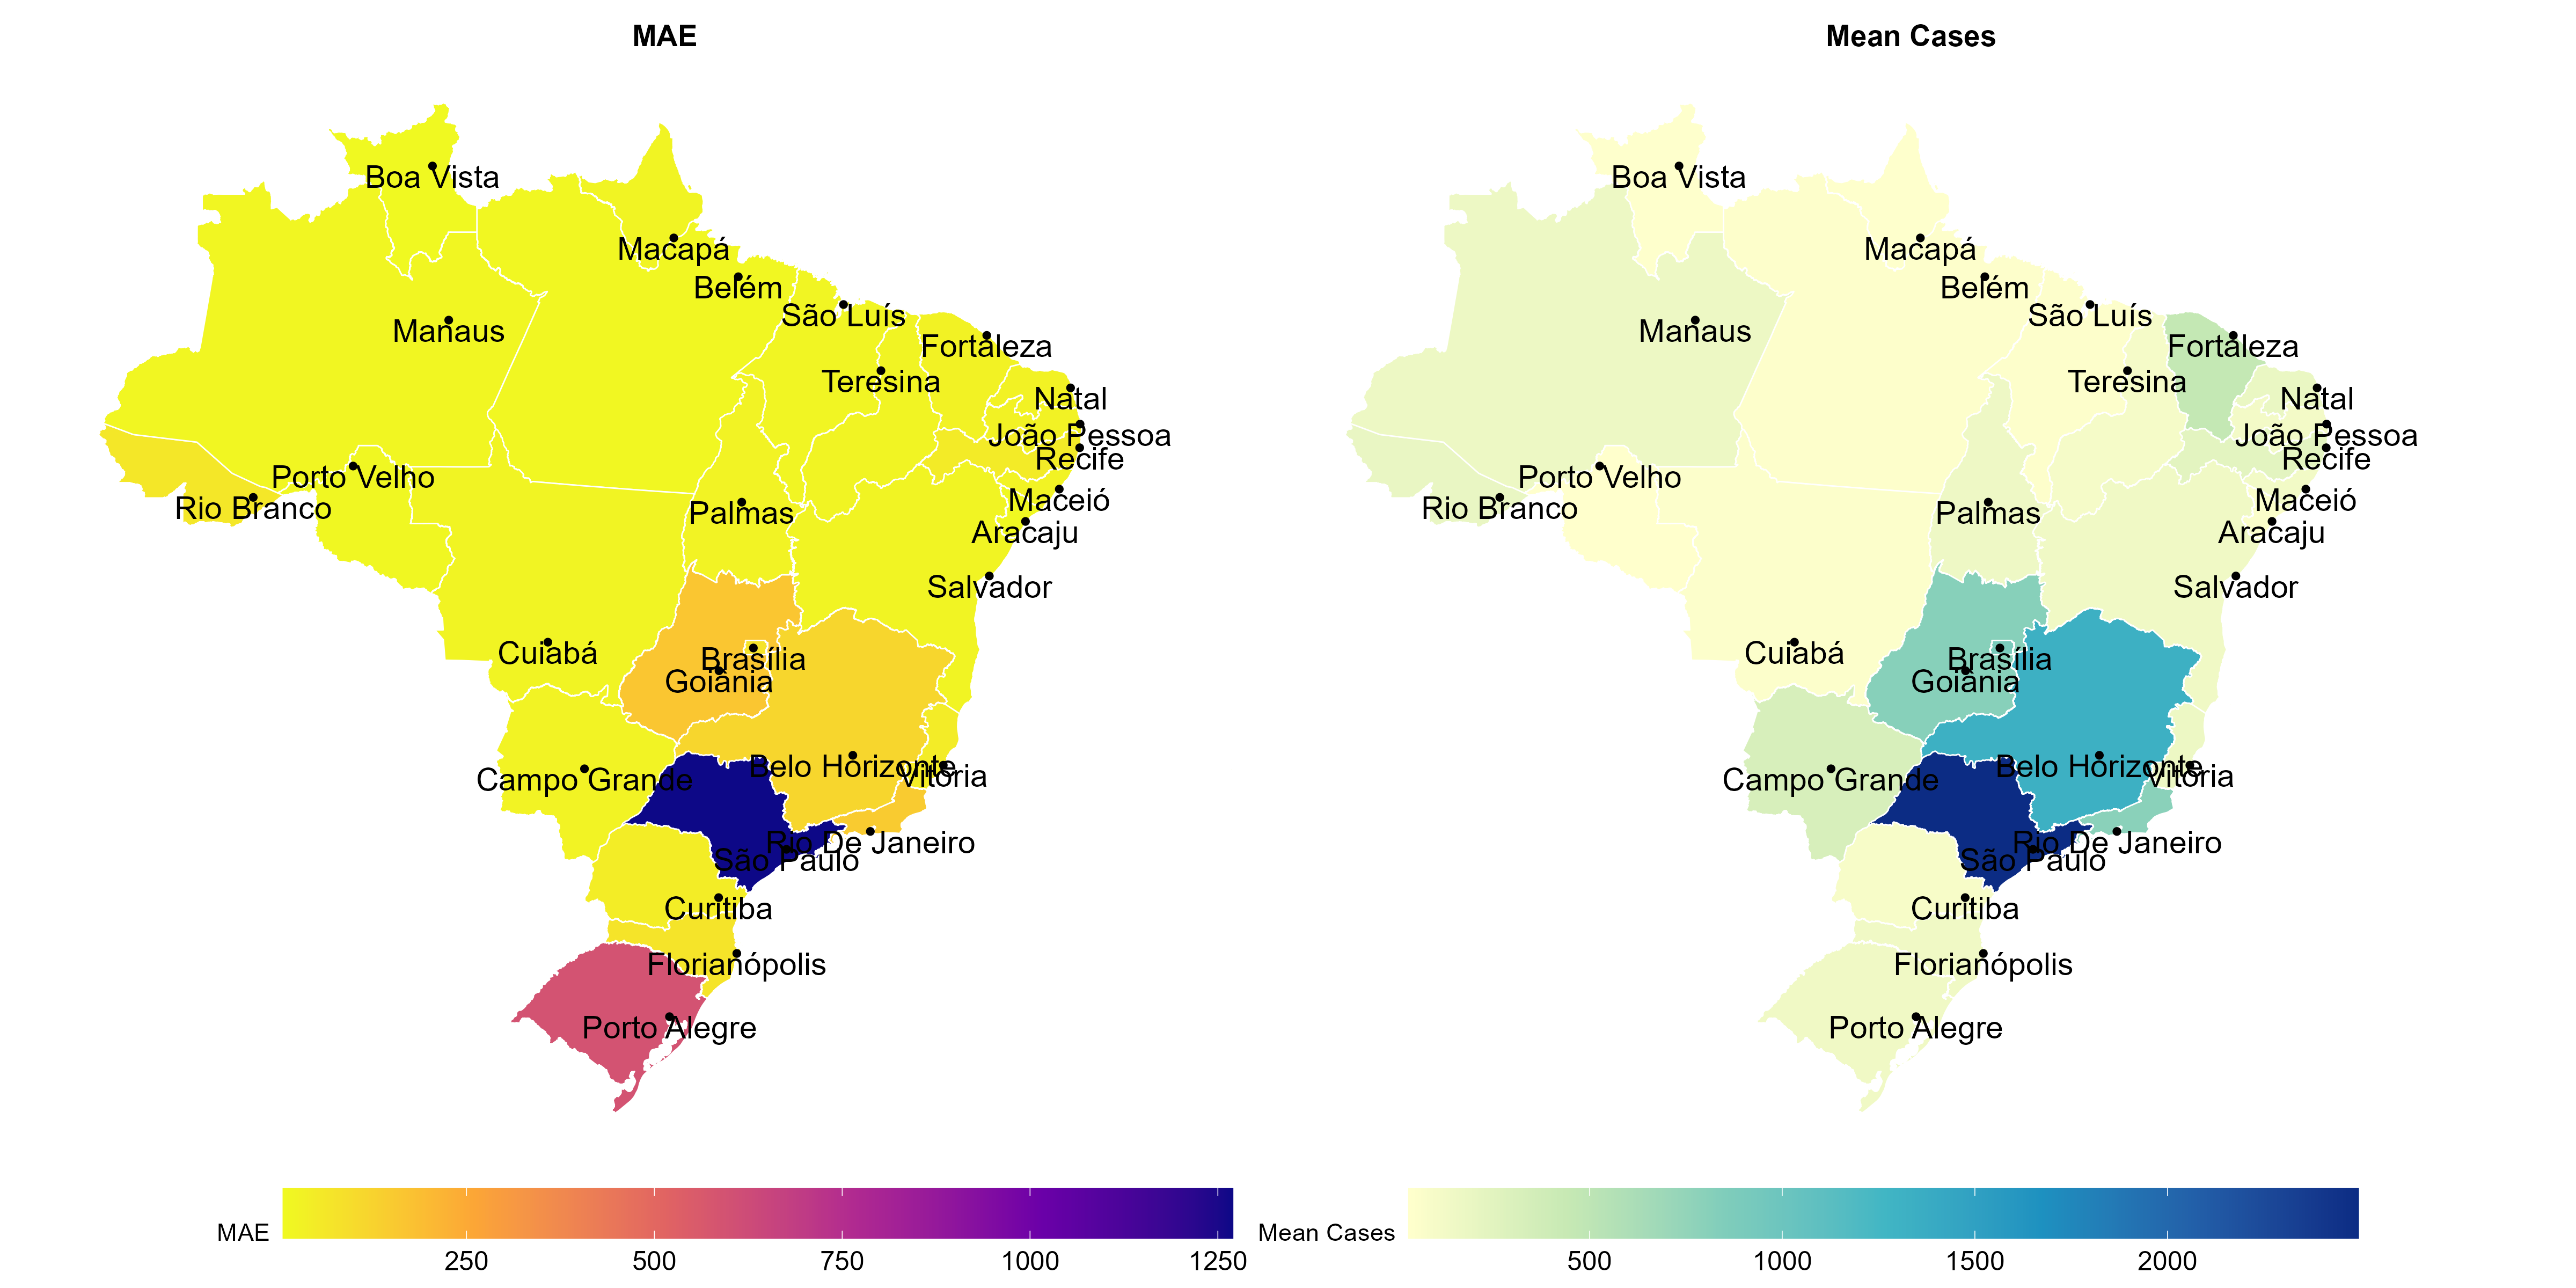
\includegraphics[scale=0.33]{figures/mae_cases_combined.png}
        \caption{Comparison between the MAE and the averaged number of reported cases.}
        \label{fig:mae_cases_combined}
    \end{figure}

\end{frame}

\begin{frame}[c]{Capital Cities Study}{Forecast accuracy highlights}

    \begin{table}[H]
        \centering
        \begin{tabular}{lcl|lcl}
            \hline
            \multicolumn{3}{c|}{Lowest MAE} & \multicolumn{3}{c}{Highest MAE} \\
            \hline
            RR & M0 & 7.30 & SP & M13 & 1268.50 \\
            SE & M8 & 9.22 & RS & M6 & 593.22 \\
            RO & M8 & 12.71 & GO & M1 & 164.33 \\
            PA & M1 & 14.90 & RJ & M3 & 149.56 \\
            \hline
        \end{tabular}
        \caption{Best models for the four lowest and highest MAE.}
    \end{table}

\end{frame}

\begin{frame}[c]{Capital Cities Study}{Forecast accuracy highlights}

    \begin{figure}
        \centering
        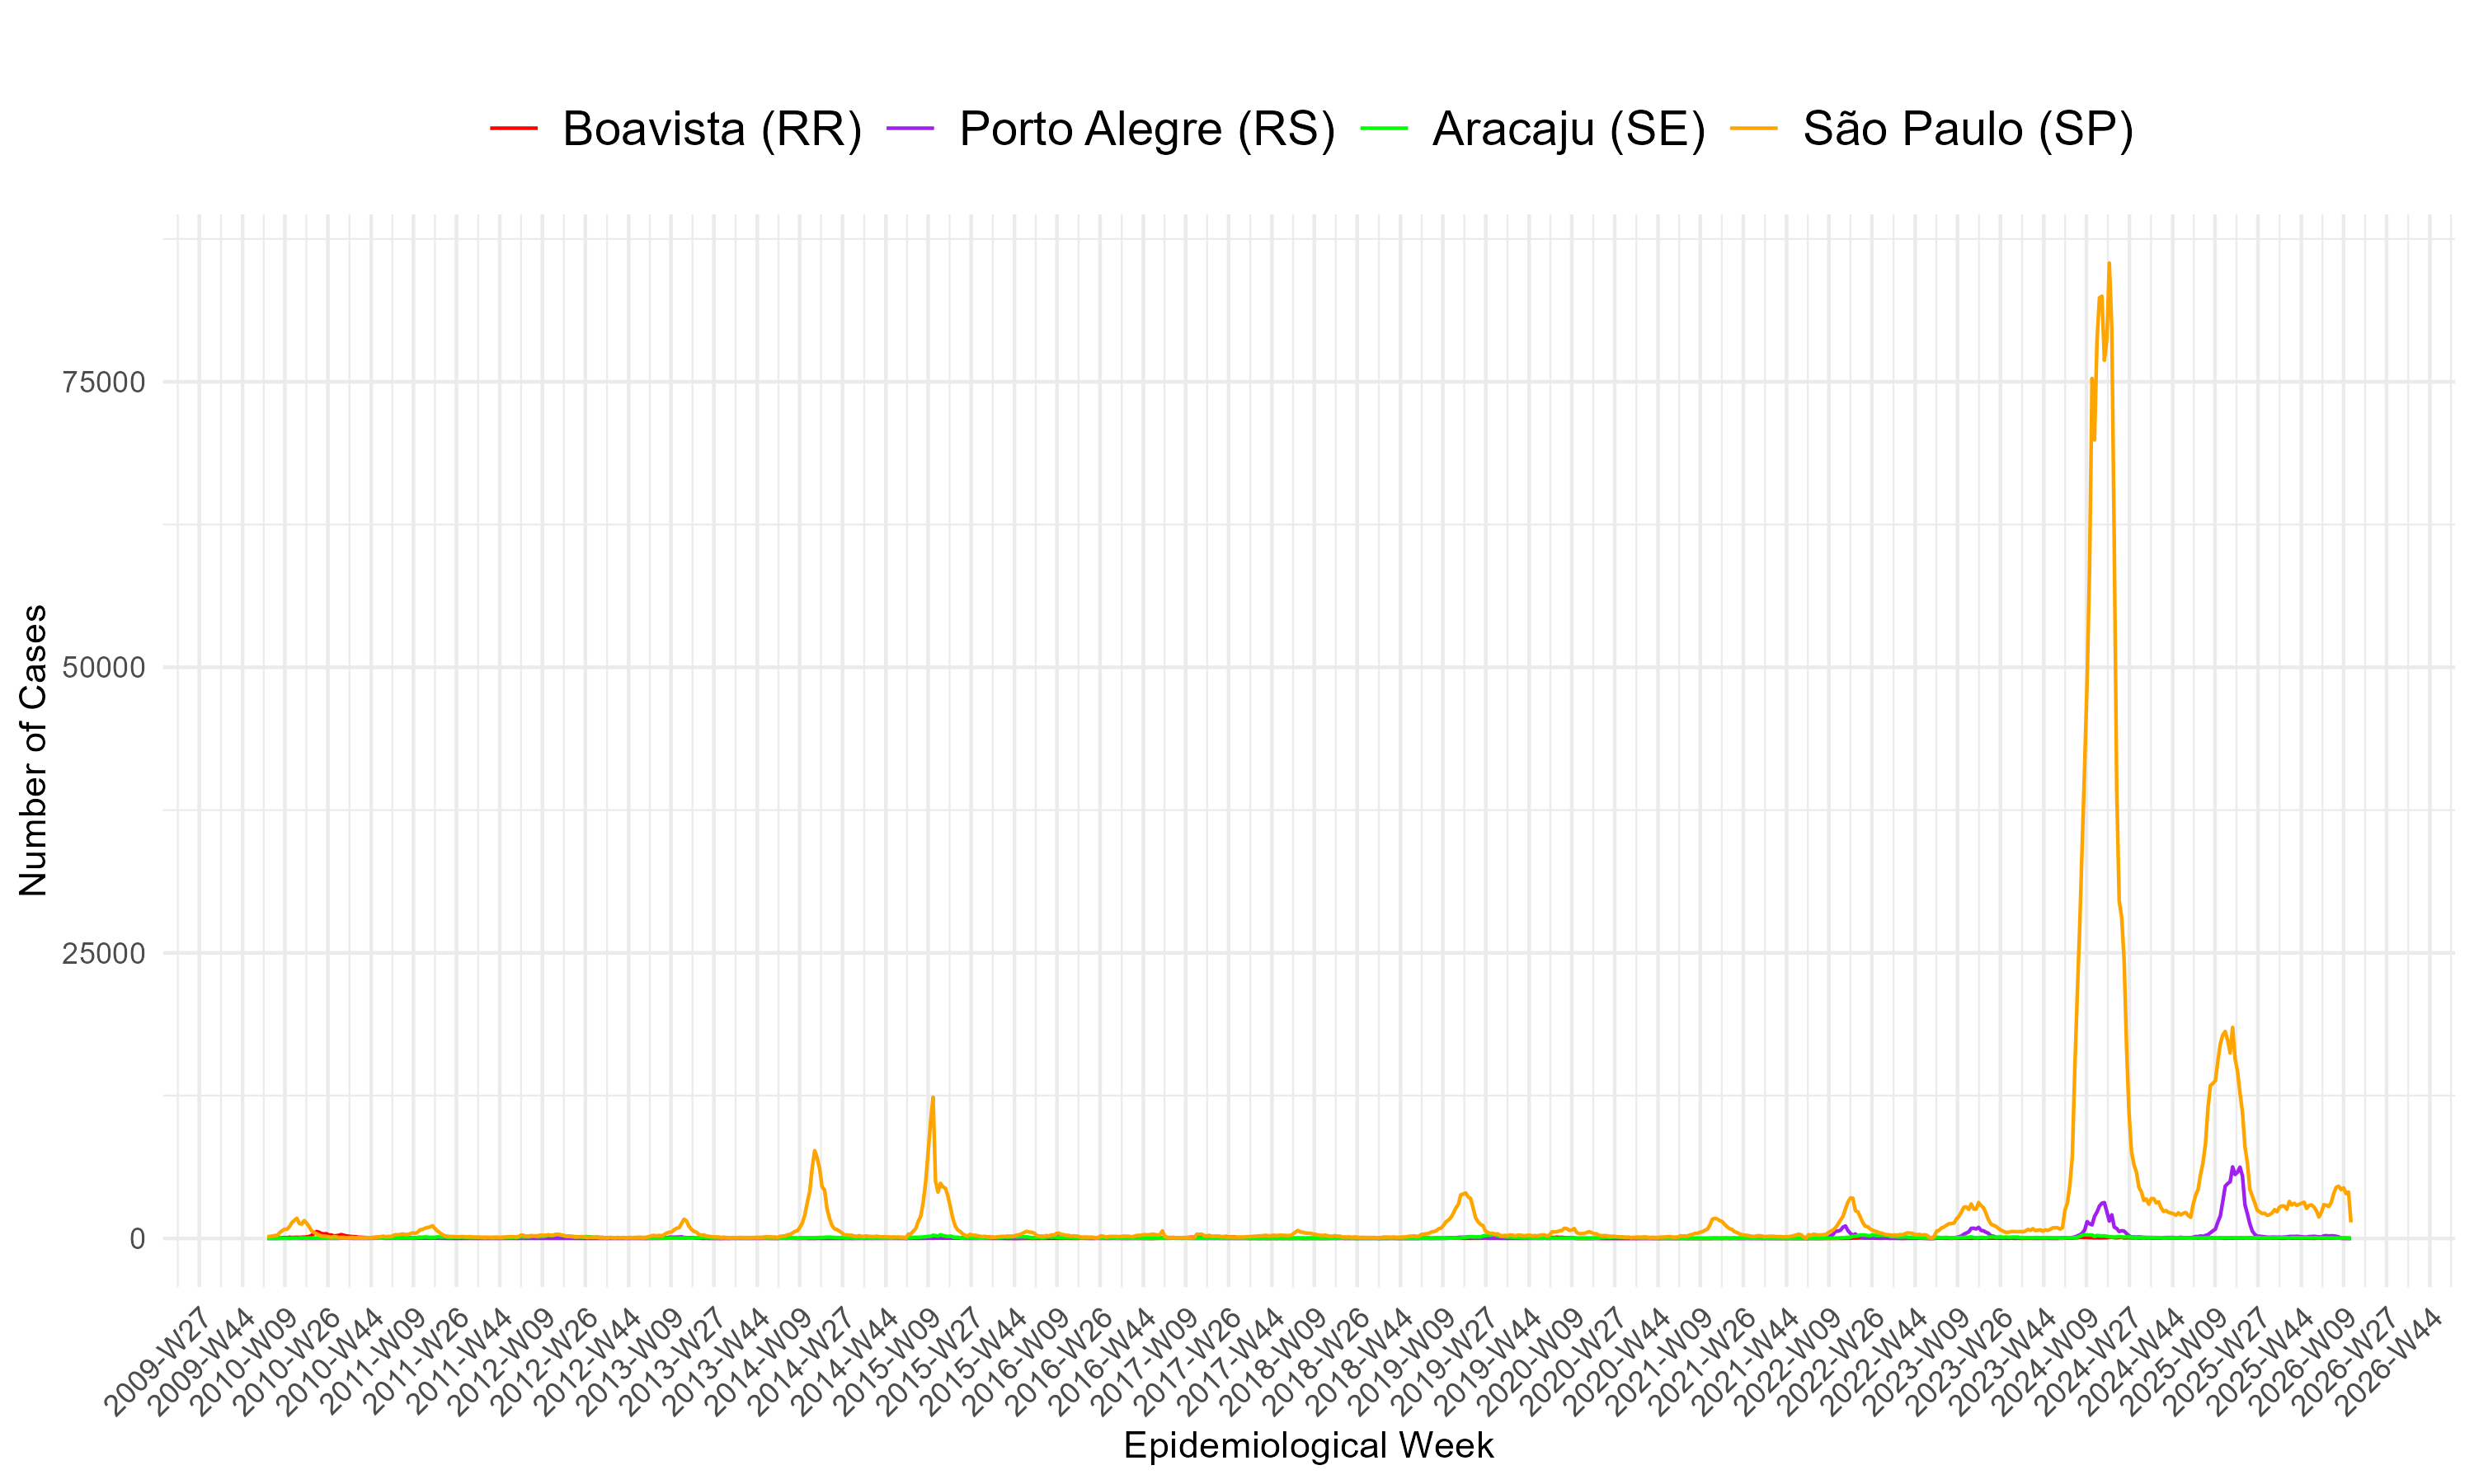
\includegraphics[scale=0.45]{figures/time_series_low_high_mae.png}
        \caption{Cases time series for selected capitals.}
        \label{fig:time_series_low_high_mae}
    \end{figure}

\end{frame}

\begin{frame}[c]{Capital Cities Study}{Key findings}

    \begin{display}[Take-away messages]
        \begin{itemize}
            \item Based on WIS, SARIMAX seems to be a more universal best model, but in general, there is \highlight{no universal best model} across the Brazilian capitals;
            \item Climate information improves forecasting in all southern capitals, but there is no clear pattern in the other regions;
            \item Highest MAEs occur in capitals with highest number of cases/peaks.
            \item In several cities, WIS leads to different choices of best models compared to MAE, especially in INLA models.
        \end{itemize}
    \end{display}

\end{frame}

\begin{frame}[c]{Capital Cities Study}{Next steps}

    \begin{itemize}
        \item Implement machine learning models;
        \item Explore regional patterns in the winning models;
    \end{itemize}

\end{frame}


\nocite{*}
% \begin{frame}[allowframebreaks]{References}
%     \printbibliography[heading=bibintoc, title={Referências}]
% \end{frame}
\begin{frame}[c]{Code availability}

    % \bibliographystyle{plain}
    \printbibliography
    
\end{frame}

\begin{frame}[c]
  \centering
  \Huge \textbf{Thank you!}
\end{frame}

\end{document} 

